\documentclass[]{article}
\usepackage{lmodern}
\usepackage{amssymb,amsmath}
\usepackage{ifxetex,ifluatex}
\usepackage{fixltx2e} % provides \textsubscript
\ifnum 0\ifxetex 1\fi\ifluatex 1\fi=0 % if pdftex
  \usepackage[T1]{fontenc}
  \usepackage[utf8]{inputenc}
\else % if luatex or xelatex
  \ifxetex
    \usepackage{mathspec}
  \else
    \usepackage{fontspec}
  \fi
  \defaultfontfeatures{Ligatures=TeX,Scale=MatchLowercase}
\fi
% use upquote if available, for straight quotes in verbatim environments
\IfFileExists{upquote.sty}{\usepackage{upquote}}{}
% use microtype if available
\IfFileExists{microtype.sty}{%
\usepackage{microtype}
\UseMicrotypeSet[protrusion]{basicmath} % disable protrusion for tt fonts
}{}
\usepackage[margin=1in]{geometry}
\usepackage{hyperref}
\hypersetup{unicode=true,
            pdftitle={732A91 - Lab 2},
            pdfauthor={Joris van Doorn \textbar\textbar{} Weng Hang Wong},
            pdfborder={0 0 0},
            breaklinks=true}
\urlstyle{same}  % don't use monospace font for urls
\usepackage{color}
\usepackage{fancyvrb}
\newcommand{\VerbBar}{|}
\newcommand{\VERB}{\Verb[commandchars=\\\{\}]}
\DefineVerbatimEnvironment{Highlighting}{Verbatim}{commandchars=\\\{\}}
% Add ',fontsize=\small' for more characters per line
\usepackage{framed}
\definecolor{shadecolor}{RGB}{248,248,248}
\newenvironment{Shaded}{\begin{snugshade}}{\end{snugshade}}
\newcommand{\AlertTok}[1]{\textcolor[rgb]{0.94,0.16,0.16}{#1}}
\newcommand{\AnnotationTok}[1]{\textcolor[rgb]{0.56,0.35,0.01}{\textbf{\textit{#1}}}}
\newcommand{\AttributeTok}[1]{\textcolor[rgb]{0.77,0.63,0.00}{#1}}
\newcommand{\BaseNTok}[1]{\textcolor[rgb]{0.00,0.00,0.81}{#1}}
\newcommand{\BuiltInTok}[1]{#1}
\newcommand{\CharTok}[1]{\textcolor[rgb]{0.31,0.60,0.02}{#1}}
\newcommand{\CommentTok}[1]{\textcolor[rgb]{0.56,0.35,0.01}{\textit{#1}}}
\newcommand{\CommentVarTok}[1]{\textcolor[rgb]{0.56,0.35,0.01}{\textbf{\textit{#1}}}}
\newcommand{\ConstantTok}[1]{\textcolor[rgb]{0.00,0.00,0.00}{#1}}
\newcommand{\ControlFlowTok}[1]{\textcolor[rgb]{0.13,0.29,0.53}{\textbf{#1}}}
\newcommand{\DataTypeTok}[1]{\textcolor[rgb]{0.13,0.29,0.53}{#1}}
\newcommand{\DecValTok}[1]{\textcolor[rgb]{0.00,0.00,0.81}{#1}}
\newcommand{\DocumentationTok}[1]{\textcolor[rgb]{0.56,0.35,0.01}{\textbf{\textit{#1}}}}
\newcommand{\ErrorTok}[1]{\textcolor[rgb]{0.64,0.00,0.00}{\textbf{#1}}}
\newcommand{\ExtensionTok}[1]{#1}
\newcommand{\FloatTok}[1]{\textcolor[rgb]{0.00,0.00,0.81}{#1}}
\newcommand{\FunctionTok}[1]{\textcolor[rgb]{0.00,0.00,0.00}{#1}}
\newcommand{\ImportTok}[1]{#1}
\newcommand{\InformationTok}[1]{\textcolor[rgb]{0.56,0.35,0.01}{\textbf{\textit{#1}}}}
\newcommand{\KeywordTok}[1]{\textcolor[rgb]{0.13,0.29,0.53}{\textbf{#1}}}
\newcommand{\NormalTok}[1]{#1}
\newcommand{\OperatorTok}[1]{\textcolor[rgb]{0.81,0.36,0.00}{\textbf{#1}}}
\newcommand{\OtherTok}[1]{\textcolor[rgb]{0.56,0.35,0.01}{#1}}
\newcommand{\PreprocessorTok}[1]{\textcolor[rgb]{0.56,0.35,0.01}{\textit{#1}}}
\newcommand{\RegionMarkerTok}[1]{#1}
\newcommand{\SpecialCharTok}[1]{\textcolor[rgb]{0.00,0.00,0.00}{#1}}
\newcommand{\SpecialStringTok}[1]{\textcolor[rgb]{0.31,0.60,0.02}{#1}}
\newcommand{\StringTok}[1]{\textcolor[rgb]{0.31,0.60,0.02}{#1}}
\newcommand{\VariableTok}[1]{\textcolor[rgb]{0.00,0.00,0.00}{#1}}
\newcommand{\VerbatimStringTok}[1]{\textcolor[rgb]{0.31,0.60,0.02}{#1}}
\newcommand{\WarningTok}[1]{\textcolor[rgb]{0.56,0.35,0.01}{\textbf{\textit{#1}}}}
\usepackage{longtable,booktabs}
\usepackage{graphicx,grffile}
\makeatletter
\def\maxwidth{\ifdim\Gin@nat@width>\linewidth\linewidth\else\Gin@nat@width\fi}
\def\maxheight{\ifdim\Gin@nat@height>\textheight\textheight\else\Gin@nat@height\fi}
\makeatother
% Scale images if necessary, so that they will not overflow the page
% margins by default, and it is still possible to overwrite the defaults
% using explicit options in \includegraphics[width, height, ...]{}
\setkeys{Gin}{width=\maxwidth,height=\maxheight,keepaspectratio}
\IfFileExists{parskip.sty}{%
\usepackage{parskip}
}{% else
\setlength{\parindent}{0pt}
\setlength{\parskip}{6pt plus 2pt minus 1pt}
}
\setlength{\emergencystretch}{3em}  % prevent overfull lines
\providecommand{\tightlist}{%
  \setlength{\itemsep}{0pt}\setlength{\parskip}{0pt}}
\setcounter{secnumdepth}{0}
% Redefines (sub)paragraphs to behave more like sections
\ifx\paragraph\undefined\else
\let\oldparagraph\paragraph
\renewcommand{\paragraph}[1]{\oldparagraph{#1}\mbox{}}
\fi
\ifx\subparagraph\undefined\else
\let\oldsubparagraph\subparagraph
\renewcommand{\subparagraph}[1]{\oldsubparagraph{#1}\mbox{}}
\fi

%%% Use protect on footnotes to avoid problems with footnotes in titles
\let\rmarkdownfootnote\footnote%
\def\footnote{\protect\rmarkdownfootnote}

%%% Change title format to be more compact
\usepackage{titling}

% Create subtitle command for use in maketitle
\providecommand{\subtitle}[1]{
  \posttitle{
    \begin{center}\large#1\end{center}
    }
}

\setlength{\droptitle}{-2em}

  \title{732A91 - Lab 2}
    \pretitle{\vspace{\droptitle}\centering\huge}
  \posttitle{\par}
    \author{Joris van Doorn \textbar\textbar{} Weng Hang Wong}
    \preauthor{\centering\large\emph}
  \postauthor{\par}
      \predate{\centering\large\emph}
  \postdate{\par}
    \date{18 五月 2020}


\begin{document}
\maketitle

\hypertarget{linear-and-polynomial-regression}{%
\section{1. Linear and polynomial
regression}\label{linear-and-polynomial-regression}}

\emph{The dataset TempLinkoping.txt contains daily average temperatures
(in Celcius degrees) at Malmslätt, Linköping over the course of the year
2018. The response variable is temp and the covariate is}

\[time = \frac{the\: number\: of\: days\: since\: beginning\: of\: year}{365}\]

\emph{The task is to perform a Bayesian analysis of a quadratic
regression}

\[temp=\beta_0+\beta_1*time+\beta_2*time^2+\epsilon,\epsilon\sim^{iid}N(0,\sigma^2)\]

\hypertarget{a.}{%
\subsection{a.}\label{a.}}

\emph{Determining the prior distribution of the model parameters. Use
the conjugate prior for the linear regression model. Your task is to set
the prior hyperparameters \(\mu_0, \Omega_0, \nu_0 \:and\:\sigma_0^2\)
to sensible values. Start with
\(\mu_0=(-10,100,-100)^T,\Omega_0=0.01\cdot I_3,\nu_0=4\:and\:\sigma_0^2\).
Check if this prior agrees with your prior opinions by simulating draws
from the joint prior of all parameters and for every draw compute the
regression curve. This gives a collection of regression curves, one for
each draw from the prior. Do the collection of curves look reasonable?
If not, change the prior hyperparameters until the collection of prior
regression curves agrees with your prior beliefs about the regression
curve.}

\begin{center}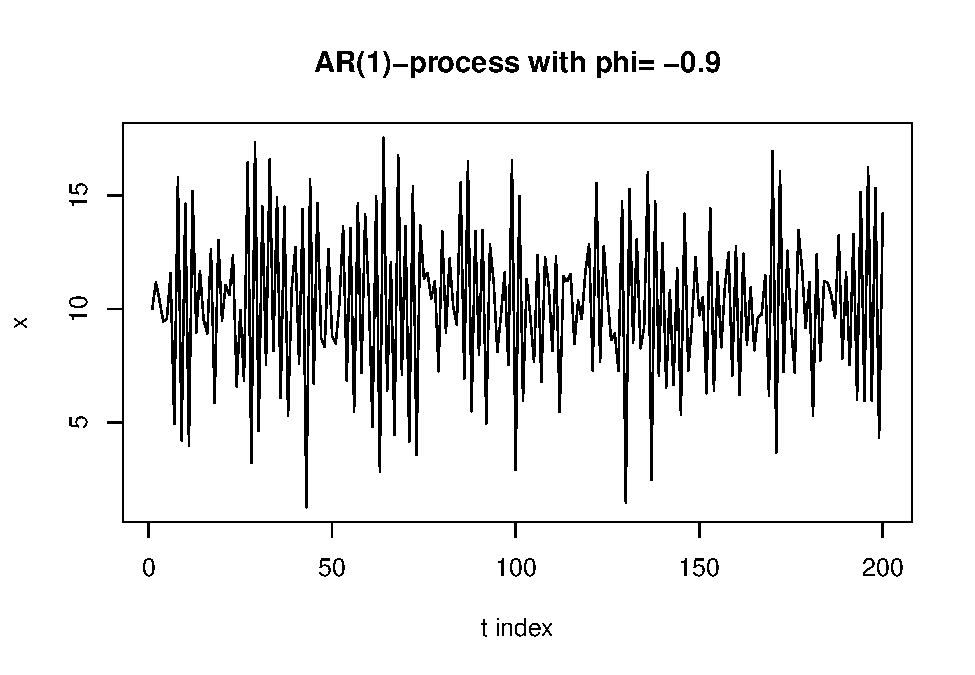
\includegraphics[width=0.8\linewidth]{732A91_lab_2_jorva845_files/figure-latex/unnamed-chunk-1-1} \end{center}

\begin{center}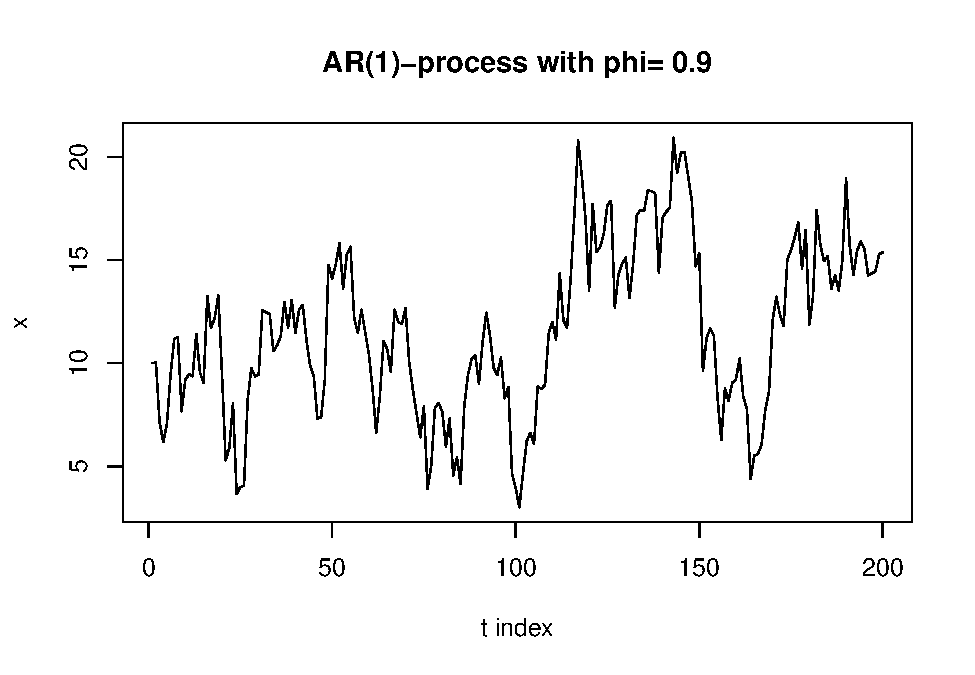
\includegraphics[width=0.8\linewidth]{732A91_lab_2_jorva845_files/figure-latex/unnamed-chunk-1-2} \end{center}

\begin{center}\includegraphics[width=0.8\linewidth]{732A91_lab_2_jorva845_files/figure-latex/unnamed-chunk-1-3} \end{center}

\hypertarget{b.}{%
\subsection{b.}\label{b.}}

\emph{Write a program that simulates from the joint posterior
distribution of \(\beta_0\),\(\beta_1\),\(\beta_2\),and \(\sigma^2\).
Plot the marginal posteriors for each parameter as a histogram. Also
produce another figure with a scatter plot of the temperature data and
overlay a curve for the posterior median of the regression function
\(f(time)=\beta_0 +\beta_1 \cdot time+\beta_2\cdot time^2\), computed
for every value of time. Also overlay curves for the lower 2.5\% and
upper 97.5\% posterior credible interval for f (time). That is, compute
the 95\% equal tail posterior probability intervals for every value of
time and then connect the lower and upper limits of the interval by
curves. Does the interval bands contain most of the data points? Should
they?}

From the graph below, the parameters are simulated from the joint
posterior distribution. The marginal posteriors for each parameter
\(\beta_0\),\(\beta_1\),\(\beta_2\),and \(\sigma^2\) are shown below.

\begin{center}\includegraphics[width=0.8\linewidth]{732A91_lab_2_jorva845_files/figure-latex/unnamed-chunk-2-1} \end{center}

\begin{center}\includegraphics[width=0.8\linewidth]{732A91_lab_2_jorva845_files/figure-latex/unnamed-chunk-2-2} \end{center}

\begin{center}\includegraphics[width=0.8\linewidth]{732A91_lab_2_jorva845_files/figure-latex/unnamed-chunk-2-3} \end{center}

\begin{center}\includegraphics[width=0.8\linewidth]{732A91_lab_2_jorva845_files/figure-latex/unnamed-chunk-2-4} \end{center}

Here is a scatter plot of the temperature data with the median and
credible interval curves. However, most of the data points are not
contained in the 95\% posterior credible interval, they should not
contained most of the data points, since it didn't include the
\(\varepsilon\) in the regression function and the uncentainty parameter
here has particular probability.

\begin{center}\includegraphics[width=0.8\linewidth]{732A91_lab_2_jorva845_files/figure-latex/unnamed-chunk-3-1} \end{center}

\hypertarget{c.}{%
\subsection{c.}\label{c.}}

\emph{It is of interest to locate the time with the highest expected
temperature (that is, the time where f (time) is maximal). Let's call
this value \(\widetilde{x}\) Use the simulations in b) to simulate from
the posterior distribution of \(\widetilde{x}\)}

The first derivative of f(time) will be maximal when it equal to zero.
\[ y= \beta_0+\beta_1\cdot x + \beta_2 \cdot x^2\]
\[0 = \beta_1 + 2\beta_2x\]
\[ \widetilde{x} = \frac{-\beta_1}{2\beta_2}\]

\begin{verbatim}
## The expected highest expected temperature is 0.5430181
\end{verbatim}

\begin{center}\includegraphics[width=0.8\linewidth]{732A91_lab_2_jorva845_files/figure-latex/unnamed-chunk-4-1} \end{center}

\hypertarget{d.}{%
\subsection{d.}\label{d.}}

\emph{Say now that you want to estimate a polynomial model of order 7,
but you suspect that higher order terms may not be needed, and you worry
about overfitting. Suggest a suitable prior that mitigates this
potential problem. You do not need to compute the posterior, just write
down your prior. {[}Hint: the task is to specify \(\mu_0\) and
\(\Omega_0\) in a smart way.{]}}

To prevent overfitting we suggest adding a regularization term. The
proposed prior would like as follows:

\[\beta_i|\sigma^2\sim^{iid}N(0,\frac{\sigma^2}{\lambda})\]

where \(\lambda\) will be the smoothness/shrinkage/regularization term.
\(\Omega_0\) and \(\lambda\) are relate as \(\Omega_0 = \lambda I\). A
change in \(\lambda\) does not directly affect \(\mu_0\). However, it
does influence \(\mu_n\) through \(\Omega_0\). The larger \(\lambda\)
is, the more shrinkage.

\newpage

\hypertarget{posterior-approximation-for-cassification-with-logistic-regression}{%
\section{2. Posterior approximation for cassification with logistic
regression}\label{posterior-approximation-for-cassification-with-logistic-regression}}

\emph{The dataset WomenWork.dat contains n = 200 observations
(i.e.~women) on the following nine variables:}

\begin{table}[]
\begin{tabular}{l|l|l|l}
Variable    & Data type & Meaning                                           & Role     \\ \hline
Work        & Binary    & Whether or not the woman works                    & Response \\
Constant    & 1         & Constant to the intercept                         & Feature  \\
HusbandInc  & Numeric   & Husband's income                                  & Feature  \\
EducYears   & Counts    & Years of education                                & Feature  \\
ExpYears    & Counts    & Years of experience                               & Feature  \\
ExpYears2   & Numeric   & (Years of experience)/10)\textasciicircum{}2      & Feature  \\
Age         & Counts    & Age                                               & Feature  \\
NSmallChild & Counts    & Number of child \textless 7 years in household    & Feature  \\
NBigChild   & Counts    & Number of child \textgreater 6 years in household & Feature 
\end{tabular}
\end{table}

\hypertarget{a.-1}{%
\subsection{a.}\label{a.-1}}

\emph{Consider the logistic regression}

\[Pr(y=1|x)=\frac{e^{x^{T}\beta}}{1+e^{x^{T}\beta}}\]

\emph{where y is the binary variable with y = 1 if the woman works and y
= 0 if she does not. x is a 8-dimensional vector containing the eight
features (including a one for the constant term that models the
intercept).} \emph{The goal is to approximate the posterior distribution
of the 8-dim parameter vector \(\beta\) with a multivariate normal
distribution}

\[\beta|y,X\sim N(\hat\beta,J_y^{-1}(\hat\beta))\]

\emph{where \(\hat\beta\) is the posterior mode and
\(J({\hat\beta}) = - \frac{\delta^2lnp(\beta|y)}{\delta\beta\delta\beta^{T}} |_{\beta={\hat\beta}}\)
is the observed Hesian evaluated at the posterior mode. Note that
\(J(\hat\beta)\) is an 8x8 matrix with second derivatives on the
diagonal and cross-derivatives
\(\frac{\delta^2lnp(\beta|y)}{\delta\beta_i\delta\beta_j}\) on the
offdiagonal. It is actually not hard to compute this derivative by hand,
but don't worry, we will let the computer do it numerically for you.
Now, both \(\hat\beta\) and \(J(\hat\beta)\) are computed by the optim
function in R. I want you to implement you own version of this. You can
use my code as a template, but I want you to write your own file so that
you understand every line of your code. Don't just copy my code. Use the
prior \(\beta\sim N(0,\tau^2I)\), with \(\tau=10\). Your report should
include your code as well as numerical values for \(\hat\beta\) and
\(J(\hat\beta)\) for the WomenWork data.}

\newpage

\emph{Compute an approximate 95\% credible interval for the variable
NSmallChild. Would you say that this feature is an important determinant
of the probability that a women works?}

\begin{longtable}[]{@{}lrrrrrrrr@{}}
\toprule
& Constant & HusbandInc & EducYears & ExpYears & ExpYears2 & Age &
NSmallChild & NBigChild\tabularnewline
\midrule
\endhead
Constant & 2.2660225 & 0.0033389 & -0.0654512 & -0.0117914 & 0.0457807 &
-0.0302934 & -0.1887484 & -0.0980239\tabularnewline
HusbandInc & 0.0033389 & 0.0002528 & -0.0005610 & -0.0000313 & 0.0001415
& -0.0000359 & 0.0005067 & -0.0001444\tabularnewline
EducYears & -0.0654512 & -0.0005610 & 0.0062182 & -0.0003558 & 0.0018963
& -0.0000032 & -0.0061346 & 0.0017527\tabularnewline
ExpYears & -0.0117914 & -0.0000313 & -0.0003558 & 0.0043517 & -0.0142491
& -0.0001341 & -0.0014690 & 0.0005437\tabularnewline
ExpYears2 & 0.0457807 & 0.0001415 & 0.0018963 & -0.0142491 & 0.0555787 &
-0.0003299 & 0.0032083 & 0.0005120\tabularnewline
Age & -0.0302934 & -0.0000359 & -0.0000032 & -0.0001341 & -0.0003299 &
0.0007185 & 0.0051842 & 0.0010953\tabularnewline
NSmallChild & -0.1887484 & 0.0005067 & -0.0061346 & -0.0014690 &
0.0032083 & 0.0051842 & 0.1512622 & 0.0067689\tabularnewline
NBigChild & -0.0980239 & -0.0001444 & 0.0017527 & 0.0005437 & 0.0005120
& 0.0010953 & 0.0067689 & 0.0199723\tabularnewline
\bottomrule
\end{longtable}

\begin{longtable}[]{@{}lrrr@{}}
\toprule
& Verification & Beta\_hat & Beta\_std\tabularnewline
\midrule
\endhead
Constant & 0.6443036 & 0.6267288 & 1.5053314\tabularnewline
HusbandInc & -0.0197746 & -0.0197911 & 0.0158998\tabularnewline
EducYears & 0.1798806 & 0.1802190 & 0.0788556\tabularnewline
ExpYears & 0.1675127 & 0.1675667 & 0.0659675\tabularnewline
ExpYears2 & -0.1443595 & -0.1445967 & 0.2357513\tabularnewline
Age & -0.0823403 & -0.0820656 & 0.0268041\tabularnewline
NSmallChild & -1.3625024 & -1.3591332 & 0.3889244\tabularnewline
NBigChild & -0.0254299 & -0.0246835 & 0.1413233\tabularnewline
\bottomrule
\end{longtable}

\begin{longtable}[]{@{}r@{}}
\toprule
NSmallChild\tabularnewline
\midrule
\endhead
-2.1141664\tabularnewline
-0.5896108\tabularnewline
\bottomrule
\end{longtable}

The number of small children seem to matter. The coefficient is by far
the largest, especial compared to the number of larger children a woman
has. This would also intuitivaly make sense, because the earlier years
of a childs life it demands more attention and it would therefore be
more likely for one of the parents to remain at home and not have a job.

\hypertarget{b.-1}{%
\subsection{b.}\label{b.-1}}

\emph{Write a function that simulates from the predictive distribution
of the response variable in a logistic regression. Use your normal
approximation from 2(a). Use that function to simulate and plot the
predictive distribution for the Work variable for a 40 year old woman,
with two children (3 and 9 years old), 8 years of education, 10 years of
experience. and a husband with an income of 10. {[}Hints: The R package
mvtnorm will again be handy. Remember my discussion on how Bayesian
prediction can be done by simulation.{]}}

\begin{center}\includegraphics[width=0.8\linewidth]{732A91_lab_2_jorva845_files/figure-latex/unnamed-chunk-6-1} \end{center}

\begin{center}\includegraphics[width=0.8\linewidth]{732A91_lab_2_jorva845_files/figure-latex/unnamed-chunk-6-2} \end{center}

\begin{verbatim}
## The expected value for this woman is:  0.515019 , thus the model predicts that she is working.
\end{verbatim}

\hypertarget{c.-1}{%
\subsection{2c.}\label{c.-1}}

\emph{Now, consider 10 women which all have the same features as the
woman in 2(b). Rewrite your function and plot the predictive
distribution for the number of women, out of these 10, that are working.
{[}Hint: Which distribution can be described as a sum of Bernoulli
random variables?{]}}

\begin{center}\includegraphics[width=0.8\linewidth]{732A91_lab_2_jorva845_files/figure-latex/unnamed-chunk-7-1} \end{center}

The binomial distribution can be approximated by a sum of bernoulli's.

\emph{!!!!2c) Analogically to 2b. This is not a predictive distribution,
you should plot a distribution in this case over 11 values (0-10 woman
working). Consider using binomial distribution!!!!!!}

\newpage

\hypertarget{appendix}{%
\section{Appendix}\label{appendix}}

\begin{Shaded}
\begin{Highlighting}[]
\NormalTok{knitr}\OperatorTok{::}\NormalTok{opts\_chunk}\OperatorTok{$}\KeywordTok{set}\NormalTok{(}\DataTypeTok{echo =} \OtherTok{TRUE}\NormalTok{)}
\NormalTok{knitr}\OperatorTok{::}\NormalTok{opts\_chunk}\OperatorTok{$}\KeywordTok{set}\NormalTok{(}\DataTypeTok{fig.width=}\DecValTok{9}\NormalTok{, }\DataTypeTok{fig.height =} \FloatTok{4.1}\NormalTok{) }
\KeywordTok{library}\NormalTok{(dplyr)}
\KeywordTok{library}\NormalTok{(knitr)}
\KeywordTok{library}\NormalTok{(mvtnorm)}
\KeywordTok{set.seed}\NormalTok{(}\DecValTok{12345}\NormalTok{)}
\CommentTok{\#{-}{-}{-}{-}{-}{-}{-}{-}{-}{-}{-}{-}{-}{-}{-}{-}{-}{-}{-}{-}{-}{-}{-}{-}{-}{-}{-}{-}{-}{-}{-}{-}{-}{-}{-}{-}{-}{-}{-}{-}{-}{-}{-}{-}{-}{-}{-}{-}{-}{-}{-}{-}{-}{-}{-}{-}{-}{-}{-}{-}{-}{-}{-}{-}{-}{-}{-}{-}{-}{-}{-}{-}{-}{-}{-}{-}{-}}
\CommentTok{\# Q1a.}
\NormalTok{data0 \textless{}{-}}\StringTok{ }\KeywordTok{read.table}\NormalTok{(}\StringTok{"TempLinkoping.txt"}\NormalTok{, }\DataTypeTok{header =} \OtherTok{TRUE}\NormalTok{)}
\NormalTok{intercept \textless{}{-}}\StringTok{ }\KeywordTok{rep}\NormalTok{(}\DecValTok{1}\NormalTok{,}\DecValTok{365}\NormalTok{)}
\NormalTok{data1 \textless{}{-}}\StringTok{ }\KeywordTok{cbind}\NormalTok{(data0, }\StringTok{"intercept"}\NormalTok{=intercept)}
\NormalTok{time2 \textless{}{-}}\StringTok{ }\NormalTok{data1}\OperatorTok{$}\NormalTok{time}\OperatorTok{\^{}}\DecValTok{2}
\NormalTok{data1 \textless{}{-}}\StringTok{ }\KeywordTok{cbind}\NormalTok{(data1, }\StringTok{"time2"}\NormalTok{=time2)}

\CommentTok{\#given hyperparameters}
\NormalTok{mu0=}\KeywordTok{matrix}\NormalTok{(}\KeywordTok{c}\NormalTok{(}\OperatorTok{{-}}\DecValTok{10}\NormalTok{,}\DecValTok{100}\NormalTok{,}\OperatorTok{{-}}\DecValTok{100}\NormalTok{))}
\NormalTok{omega0=}\KeywordTok{diag}\NormalTok{(}\DataTypeTok{x=}\FloatTok{0.01}\NormalTok{, }\DataTypeTok{nrow=}\DecValTok{3}\NormalTok{, }\DataTypeTok{ncol=}\DecValTok{3}\NormalTok{)}
\NormalTok{v0=}\DecValTok{4}
\NormalTok{sigma20=}\DecValTok{1}

\CommentTok{\#prior}
\NormalTok{PriorReg =}\StringTok{ }\ControlFlowTok{function}\NormalTok{(mu0,omega0,v0,sigma20)\{}
  \KeywordTok{set.seed}\NormalTok{(}\DecValTok{12345}\NormalTok{)}
  \ControlFlowTok{for}\NormalTok{(i }\ControlFlowTok{in} \DecValTok{1}\OperatorTok{:}\DecValTok{100}\NormalTok{)\{}
    \CommentTok{\#using chi\_sq to sample sigma\^{}2}
\NormalTok{    chi\_sample =}\StringTok{ }\KeywordTok{rchisq}\NormalTok{(}\DataTypeTok{n=}\DecValTok{1}\NormalTok{, }\DataTypeTok{df=}\NormalTok{v0)}
\NormalTok{    sigma2 =}\StringTok{ }\NormalTok{v0}\OperatorTok{*}\NormalTok{sigma20}\OperatorTok{/}\NormalTok{chi\_sample}
    
    \CommentTok{\#using mvtnorm sample beta}
\NormalTok{    beta =}\StringTok{ }\KeywordTok{rmvnorm}\NormalTok{(}\DataTypeTok{n=}\DecValTok{1}\NormalTok{, }\DataTypeTok{mean=}\NormalTok{mu0, }\DataTypeTok{sigma=}\NormalTok{sigma20}\OperatorTok{*}\KeywordTok{solve}\NormalTok{(omega0))}
    
    \CommentTok{\#quadratic regression  }
\NormalTok{    quad\_regre=}\StringTok{ }\NormalTok{beta[}\DecValTok{1}\NormalTok{]}\OperatorTok{+}\NormalTok{beta[}\DecValTok{2}\NormalTok{]}\OperatorTok{*}\NormalTok{data0}\OperatorTok{$}\NormalTok{time}\OperatorTok{+}\NormalTok{beta[}\DecValTok{3}\NormalTok{]}\OperatorTok{*}\NormalTok{(data0}\OperatorTok{$}\NormalTok{time}\OperatorTok{\^{}}\DecValTok{2}\NormalTok{)}\OperatorTok{+}\KeywordTok{rnorm}\NormalTok{(}\DecValTok{1}\NormalTok{,}\DataTypeTok{mean=}\DecValTok{0}\NormalTok{, }\DataTypeTok{sd=}\KeywordTok{sqrt}\NormalTok{(sigma2))}
    \KeywordTok{lines}\NormalTok{(}\DataTypeTok{x=}\NormalTok{data0}\OperatorTok{$}\NormalTok{time, }\DataTypeTok{y=}\NormalTok{quad\_regre,}\DataTypeTok{col=}\StringTok{"red"}\NormalTok{,}\DataTypeTok{lwd=}\DecValTok{2}\NormalTok{)}
\NormalTok{  \}}
\NormalTok{\}}

\CommentTok{\#\#\# Check the given hyperpara}
\KeywordTok{plot}\NormalTok{(data0, }\DataTypeTok{main=}\StringTok{"Predicted Temperature with given hyperparameters"}\NormalTok{, }\DataTypeTok{ylab=}\StringTok{"Temperature"}\NormalTok{, }\DataTypeTok{xlab=}\StringTok{"Time"}\NormalTok{, }\DataTypeTok{type=}\StringTok{"l"}\NormalTok{)}
\KeywordTok{PriorReg}\NormalTok{( mu0, omega0, v0, sigma20)}

\CommentTok{\#\#\# change the hyperpara nu}
\KeywordTok{plot}\NormalTok{(data0, }\DataTypeTok{main=}\StringTok{"Predicted Temperature with given hyperparameters"}\NormalTok{, }\DataTypeTok{ylab=}\StringTok{"Temperature"}\NormalTok{, }\DataTypeTok{xlab=}\StringTok{"Time"}\NormalTok{, }\DataTypeTok{type=}\StringTok{"l"}\NormalTok{)}
\KeywordTok{PriorReg}\NormalTok{( mu0, omega0, v0, }\DataTypeTok{sigma20=}\FloatTok{0.03}\NormalTok{)}


\CommentTok{\# Change the hyperpara sigma}
\KeywordTok{plot}\NormalTok{(data0, }\DataTypeTok{main=}\StringTok{"Predicted Temperature with changed hyperparameters"}\NormalTok{, }\DataTypeTok{ylab=}\StringTok{"Temperature"}\NormalTok{, }\DataTypeTok{xlab=}\StringTok{"Time"}\NormalTok{, }\DataTypeTok{type=}\StringTok{"l"}\NormalTok{)}
\KeywordTok{PriorReg}\NormalTok{( }\DataTypeTok{mu0=}\KeywordTok{matrix}\NormalTok{(}\KeywordTok{c}\NormalTok{(}\OperatorTok{{-}}\DecValTok{10}\NormalTok{,}\DecValTok{110}\NormalTok{,}\OperatorTok{{-}}\DecValTok{105}\NormalTok{)), omega0, v0, }\DataTypeTok{sigma20=}\FloatTok{0.03}\NormalTok{)}
\CommentTok{\#{-}{-}{-}{-}{-}{-}{-}{-}{-}{-}{-}{-}{-}{-}{-}{-}{-}{-}{-}{-}{-}{-}{-}{-}{-}{-}{-}{-}{-}{-}{-}{-}{-}{-}{-}{-}{-}{-}{-}{-}{-}{-}{-}{-}{-}}
\CommentTok{\#Q1b.}

\CommentTok{\#\#\# find beta hat}
\NormalTok{n=}\KeywordTok{dim}\NormalTok{(data0)[}\DecValTok{1}\NormalTok{]}
\NormalTok{X =}\StringTok{ }\KeywordTok{data.frame}\NormalTok{(}\DataTypeTok{intercept=}\KeywordTok{rep}\NormalTok{(}\DecValTok{1}\NormalTok{,n), }\DataTypeTok{x1=}\NormalTok{data0}\OperatorTok{$}\NormalTok{time, }\DataTypeTok{x2=}\NormalTok{data0}\OperatorTok{$}\NormalTok{time}\OperatorTok{\^{}}\DecValTok{2}\NormalTok{)}
\NormalTok{X =}\StringTok{ }\KeywordTok{as.matrix}\NormalTok{(X)}
\NormalTok{y =}\StringTok{ }\NormalTok{data0}\OperatorTok{$}\NormalTok{temp}
\NormalTok{betaHat =}\StringTok{ }\KeywordTok{solve}\NormalTok{(}\KeywordTok{t}\NormalTok{(X)}\OperatorTok{\%*\%}\NormalTok{X)}\OperatorTok{\%*\%}\KeywordTok{t}\NormalTok{(X)}\OperatorTok{\%*\%}\NormalTok{y}

\CommentTok{\#\#\# calculate mu, omega, nu sigma}
\NormalTok{mu\_n =}\StringTok{ }\KeywordTok{solve}\NormalTok{(}\KeywordTok{t}\NormalTok{(X)}\OperatorTok{\%*\%}\NormalTok{X}\OperatorTok{+}\NormalTok{omega0) }\OperatorTok{\%*\%}\StringTok{ }\NormalTok{(}\KeywordTok{t}\NormalTok{(X)}\OperatorTok{\%*\%}\NormalTok{X}\OperatorTok{\%*\%}\NormalTok{betaHat}\OperatorTok{+}\NormalTok{omega0}\OperatorTok{\%*\%}\NormalTok{mu0)}
\NormalTok{omega\_n =}\StringTok{ }\KeywordTok{t}\NormalTok{(X)}\OperatorTok{\%*\%}\NormalTok{X}\OperatorTok{+}\NormalTok{omega0}
\NormalTok{v\_n =}\StringTok{ }\NormalTok{v0 }\OperatorTok{+}\StringTok{ }\NormalTok{n}
\NormalTok{sigma2\_n =}\StringTok{ }\NormalTok{(v0}\OperatorTok{*}\NormalTok{sigma20}\OperatorTok{+}\NormalTok{(}\KeywordTok{t}\NormalTok{(y)}\OperatorTok{\%*\%}\NormalTok{y}\OperatorTok{+}\KeywordTok{t}\NormalTok{(mu0)}\OperatorTok{\%*\%}\NormalTok{omega0}\OperatorTok{\%*\%}\NormalTok{mu0}\OperatorTok{{-}}\KeywordTok{t}\NormalTok{(mu\_n)}\OperatorTok{\%*\%}\NormalTok{omega\_n}\OperatorTok{\%*\%}\NormalTok{mu\_n))}\OperatorTok{/}\NormalTok{v\_n}

\CommentTok{\#\#\# Marginal posterior }
\KeywordTok{set.seed}\NormalTok{(}\DecValTok{12345}\NormalTok{)}
\NormalTok{paras =}\StringTok{ }\OtherTok{NULL}
\NormalTok{final =}\StringTok{ }\OtherTok{NULL}
\ControlFlowTok{for}\NormalTok{(i }\ControlFlowTok{in} \DecValTok{1}\OperatorTok{:}\DecValTok{1000}\NormalTok{)\{}
  \CommentTok{\#using chi\_sq to sample posterior sigma\^{}2}
\NormalTok{  chi\_sample =}\StringTok{ }\KeywordTok{rchisq}\NormalTok{(}\DataTypeTok{n=}\DecValTok{1}\NormalTok{, }\DataTypeTok{df=}\NormalTok{v\_n)}
\NormalTok{  post\_sigma2 =}\StringTok{ }\NormalTok{v\_n}\OperatorTok{*}\NormalTok{sigma2\_n}\OperatorTok{/}\NormalTok{chi\_sample}
  
  \CommentTok{\#using mvtnorm sample posterior beta}
\NormalTok{  post\_beta =}\StringTok{ }\KeywordTok{rmvnorm}\NormalTok{(}\DataTypeTok{n=}\DecValTok{1}\NormalTok{, }\DataTypeTok{mean=}\NormalTok{mu\_n, }\DataTypeTok{sigma=}\NormalTok{post\_sigma2[}\DecValTok{1}\NormalTok{]}\OperatorTok{*}\KeywordTok{solve}\NormalTok{(omega\_n))}
  
\NormalTok{  paras =}\StringTok{ }\KeywordTok{cbind}\NormalTok{(post\_beta,post\_sigma2)}
\NormalTok{  final =}\StringTok{ }\KeywordTok{rbind}\NormalTok{(paras, final)}
\NormalTok{\}}

\KeywordTok{colnames}\NormalTok{(final) =}\StringTok{ }\KeywordTok{c}\NormalTok{(}\StringTok{"beta0"}\NormalTok{,}\StringTok{"beta1"}\NormalTok{,}\StringTok{"beta2"}\NormalTok{,}\StringTok{"sigma2"}\NormalTok{)}

\CommentTok{\#\# histogram of each parameters}
\KeywordTok{hist}\NormalTok{(final[,}\DecValTok{1}\NormalTok{], }\DataTypeTok{main=}\StringTok{"beta 0"}\NormalTok{, }\DataTypeTok{xlab=}\StringTok{"Beta value"}\NormalTok{, }\DataTypeTok{breaks=}\DecValTok{30}\NormalTok{)}
\KeywordTok{hist}\NormalTok{(final[,}\DecValTok{2}\NormalTok{], }\DataTypeTok{main=}\StringTok{"beta 1"}\NormalTok{, }\DataTypeTok{xlab=}\StringTok{"Beta value"}\NormalTok{, }\DataTypeTok{breaks=}\DecValTok{30}\NormalTok{)}
\KeywordTok{hist}\NormalTok{(final[,}\DecValTok{3}\NormalTok{], }\DataTypeTok{main=}\StringTok{"beta 2"}\NormalTok{, }\DataTypeTok{xlab=}\StringTok{"Beta value"}\NormalTok{, }\DataTypeTok{breaks=}\DecValTok{30}\NormalTok{)}
\KeywordTok{hist}\NormalTok{(final[,}\DecValTok{4}\NormalTok{], }\DataTypeTok{main=}\StringTok{"Sigma\^{}2"}\NormalTok{,}\DataTypeTok{xlab=}\StringTok{"Sigma\^{}2 value"}\NormalTok{, }\DataTypeTok{breaks=}\DecValTok{30}\NormalTok{)}
\CommentTok{\#\#\# median curve and intervals}
\NormalTok{post\_beta =}\StringTok{ }\NormalTok{final[,}\DecValTok{1}\OperatorTok{:}\DecValTok{3}\NormalTok{]}

\NormalTok{PredictedVal=}\KeywordTok{matrix}\NormalTok{(}\DecValTok{0}\NormalTok{,}\DataTypeTok{nrow=}\NormalTok{n,}\DataTypeTok{ncol=}\KeywordTok{nrow}\NormalTok{(post\_beta))}
\ControlFlowTok{for}\NormalTok{(i }\ControlFlowTok{in} \DecValTok{1}\OperatorTok{:}\KeywordTok{nrow}\NormalTok{(post\_beta))\{}
\NormalTok{  PredictedVal[,i] =}\StringTok{ }\NormalTok{X }\OperatorTok{\%*\%}\StringTok{ }\NormalTok{post\_beta[i,]}
\NormalTok{\}}

\CommentTok{\#\# find median and credible interval}
\NormalTok{medianInterval=}\KeywordTok{c}\NormalTok{()}
\NormalTok{crediInterval =}\StringTok{ }\KeywordTok{matrix}\NormalTok{(}\DecValTok{0}\NormalTok{,}\DataTypeTok{nrow=}\NormalTok{n,}\DataTypeTok{ncol=}\DecValTok{2}\NormalTok{)}
\ControlFlowTok{for}\NormalTok{(i }\ControlFlowTok{in} \DecValTok{1}\OperatorTok{:}\NormalTok{n)\{}
\NormalTok{  medianInterval[i] =}\StringTok{ }\KeywordTok{median}\NormalTok{(PredictedVal[i,])}
\NormalTok{  crediInterval[i,] =}\StringTok{ }\KeywordTok{quantile}\NormalTok{(PredictedVal[i,], }\KeywordTok{c}\NormalTok{(}\FloatTok{0.025}\NormalTok{,}\FloatTok{0.975}\NormalTok{))}

\NormalTok{\}}

\KeywordTok{plot}\NormalTok{(data0, }\DataTypeTok{main=}\StringTok{"Predicted Interval Curves"}\NormalTok{, }\DataTypeTok{col=}\StringTok{"darkgrey"}\NormalTok{, }\DataTypeTok{ylab=}\StringTok{"temperature"}\NormalTok{)}
\KeywordTok{lines}\NormalTok{(data0}\OperatorTok{$}\NormalTok{time,medianInterval, }\DataTypeTok{col=}\StringTok{"pink"}\NormalTok{,}\DataTypeTok{lwd=}\DecValTok{2}\NormalTok{)}
\KeywordTok{lines}\NormalTok{(data0}\OperatorTok{$}\NormalTok{time,crediInterval[,}\DecValTok{1}\NormalTok{], }\DataTypeTok{col=}\StringTok{"blue"}\NormalTok{,}\DataTypeTok{lwd=}\DecValTok{2}\NormalTok{)}
\KeywordTok{lines}\NormalTok{(data0}\OperatorTok{$}\NormalTok{time,crediInterval[,}\DecValTok{2}\NormalTok{], }\DataTypeTok{col=}\StringTok{"blue"}\NormalTok{,}\DataTypeTok{lwd=}\DecValTok{2}\NormalTok{)}
\KeywordTok{legend}\NormalTok{(}\StringTok{"bottomright"}\NormalTok{,}\DataTypeTok{legend=}\KeywordTok{c}\NormalTok{(}\StringTok{"Median"}\NormalTok{, }\StringTok{"Credible Interval"}\NormalTok{), }\DataTypeTok{col=}\KeywordTok{c}\NormalTok{(}\StringTok{"pink"}\NormalTok{,}\StringTok{"blue"}\NormalTok{),}\DataTypeTok{lwd=}\DecValTok{2}\NormalTok{ )}

\CommentTok{\#{-}{-}{-}{-}{-}{-}{-}{-}{-}{-}{-}{-}{-}{-}{-}{-}{-}{-}{-}{-}{-}{-}{-}{-}{-}{-}{-}{-}{-}{-}{-}{-}{-}{-}{-}{-}{-}{-}{-}{-}{-}{-}{-}{-}{-}{-}{-}{-}{-}{-}{-}{-}{-}{-}{-}{-}{-}{-}{-}{-}{-}{-}}
\CommentTok{\#Q1c.}

\NormalTok{x\_tilde =}\StringTok{ }\OperatorTok{{-}}\NormalTok{post\_beta[,}\DecValTok{2}\NormalTok{]}\OperatorTok{/}\StringTok{ }\NormalTok{(}\DecValTok{2}\OperatorTok{*}\NormalTok{post\_beta[,}\DecValTok{3}\NormalTok{])}
\KeywordTok{cat}\NormalTok{(}\StringTok{"The expected highest expected temperature is"}\NormalTok{,}\KeywordTok{mean}\NormalTok{(x\_tilde))}

\KeywordTok{hist}\NormalTok{(x\_tilde, }\DataTypeTok{freq=}\NormalTok{F, }\DataTypeTok{breaks=}\DecValTok{20}\NormalTok{)}

\CommentTok{\# {-}{-}{-}{-}{-}{-}{-}{-}{-}{-}{-}{-}{-}{-}{-}{-}{-}{-}{-}{-}{-}{-}{-}{-}{-}}
\CommentTok{\# Q2a.}

\CommentTok{\# loading data}
\NormalTok{data0 \textless{}{-}}\StringTok{ }\KeywordTok{read.table}\NormalTok{(}\StringTok{"WomenWork.dat"}\NormalTok{,}\DataTypeTok{header =}\NormalTok{ T)}

\CommentTok{\# setting initial values}
\NormalTok{tau \textless{}{-}}\StringTok{ }\DecValTok{10} 
\NormalTok{y \textless{}{-}}\StringTok{ }\NormalTok{data0[,}\DecValTok{1}\NormalTok{]}
\NormalTok{X \textless{}{-}}\StringTok{ }\KeywordTok{as.matrix}\NormalTok{(data0[,}\DecValTok{2}\OperatorTok{:}\DecValTok{9}\NormalTok{])}
\NormalTok{nCov \textless{}{-}}\StringTok{ }\KeywordTok{dim}\NormalTok{(X)[}\DecValTok{2}\NormalTok{]}
\NormalTok{covNames \textless{}{-}}\StringTok{ }\KeywordTok{names}\NormalTok{(data0)[}\DecValTok{2}\OperatorTok{:}\DecValTok{9}\NormalTok{]}

\CommentTok{\# Prior}
\NormalTok{mu \textless{}{-}}\StringTok{ }\KeywordTok{as.vector}\NormalTok{(}\KeywordTok{rep}\NormalTok{(}\DecValTok{0}\NormalTok{,nCov))}
\NormalTok{sigma \textless{}{-}}\StringTok{ }\NormalTok{tau}\OperatorTok{\^{}}\DecValTok{2}\OperatorTok{*}\KeywordTok{diag}\NormalTok{(nCov)}

\KeywordTok{set.seed}\NormalTok{(}\DecValTok{12345}\NormalTok{)}
\CommentTok{\# Logistic regression function that returns the regression coefficients}
\NormalTok{logiPost \textless{}{-}}\StringTok{ }\ControlFlowTok{function}\NormalTok{(betas,y,X,sigma)\{}
\NormalTok{  pred \textless{}{-}}\StringTok{ }\KeywordTok{as.vector}\NormalTok{(X}\OperatorTok{\%*\%}\NormalTok{betas)}
\NormalTok{  loglike \textless{}{-}}\StringTok{ }\KeywordTok{sum}\NormalTok{(y}\OperatorTok{*}\NormalTok{pred}\OperatorTok{{-}}\KeywordTok{log}\NormalTok{(}\DecValTok{1}\OperatorTok{+}\KeywordTok{exp}\NormalTok{(pred)))}
\NormalTok{  logprior \textless{}{-}}\StringTok{ }\KeywordTok{dmvnorm}\NormalTok{(betas, }\DataTypeTok{mean=}\KeywordTok{rep}\NormalTok{(}\DecValTok{0}\NormalTok{,}\KeywordTok{length}\NormalTok{(betas)), sigma, }\DataTypeTok{log=}\NormalTok{T)}
  \KeywordTok{return}\NormalTok{(loglike}\OperatorTok{+}\NormalTok{logprior)}
\NormalTok{\}}

\CommentTok{\# setting initial values}
\NormalTok{initVal \textless{}{-}}\StringTok{ }\KeywordTok{as.vector}\NormalTok{(}\KeywordTok{rep}\NormalTok{(}\DecValTok{0}\NormalTok{,nCov)) }
\CommentTok{\# optimize over the betas}
\NormalTok{optRes \textless{}{-}}\StringTok{ }\KeywordTok{optim}\NormalTok{(initVal,logiPost,}\DataTypeTok{gr=}\OtherTok{NULL}\NormalTok{,y,X,sigma,}\DataTypeTok{method=}\StringTok{"BFGS"}\NormalTok{,}\DataTypeTok{control=}\KeywordTok{list}\NormalTok{(}\DataTypeTok{fnscale=}\OperatorTok{{-}}\DecValTok{1}\NormalTok{),}\DataTypeTok{hessian=}\NormalTok{T)}

\CommentTok{\# retrieving betas }
\NormalTok{beta\_hat \textless{}{-}}\StringTok{ }\NormalTok{optRes}\OperatorTok{$}\NormalTok{par}
\NormalTok{beta\_hes \textless{}{-}}\StringTok{ }\OperatorTok{{-}}\KeywordTok{solve}\NormalTok{(optRes}\OperatorTok{$}\NormalTok{hessian)}
\NormalTok{beta\_std \textless{}{-}}\StringTok{ }\KeywordTok{as.matrix}\NormalTok{(}\KeywordTok{sqrt}\NormalTok{(}\KeywordTok{diag}\NormalTok{(beta\_hes)))}

\CommentTok{\# verifing results}
\NormalTok{model0 \textless{}{-}}\StringTok{ }\KeywordTok{glm}\NormalTok{(Work}\OperatorTok{\textasciitilde{}}\DecValTok{0}\OperatorTok{+}\NormalTok{., }\DataTypeTok{data=}\NormalTok{data0, }\DataTypeTok{family=}\NormalTok{binomial)}

\CommentTok{\# printing results}
\KeywordTok{colnames}\NormalTok{(beta\_hes) \textless{}{-}}\StringTok{ }\NormalTok{covNames}
\KeywordTok{rownames}\NormalTok{(beta\_hes) \textless{}{-}}\StringTok{ }\NormalTok{covNames}
\KeywordTok{kable}\NormalTok{(beta\_hes)}

\KeywordTok{kable}\NormalTok{(}\KeywordTok{data.frame}\NormalTok{(}\DataTypeTok{Verification=}\NormalTok{model0}\OperatorTok{$}\NormalTok{coefficients,}\DataTypeTok{Beta\_hat=}\NormalTok{beta\_hat,}\DataTypeTok{Beta\_std=}\NormalTok{beta\_std))}


\CommentTok{\#set.seed(12345)}
\CommentTok{\#Small\_beta\_hat \textless{}{-} rmvnorm(n=1000, mean=beta\_hat, sigma = beta\_hes)}
\CommentTok{\#CI\_NSmallChild \textless{}{-} c(qnorm(0.025,mean=mean(Small\_beta\_hat[,7]),sd=beta\_std[7]),qnorm(0.975,mean=mean(Small\_beta\_hat[,7]),sd=beta\_std[7]))}

\CommentTok{\#\# find the CI for NSmallChild by simulating from the Post}
\KeywordTok{set.seed}\NormalTok{(}\DecValTok{12345}\NormalTok{)}
\NormalTok{Post\_beta\_hat =}\StringTok{ }\KeywordTok{rmvnorm}\NormalTok{(}\DataTypeTok{n=}\DecValTok{1000}\NormalTok{, }\DataTypeTok{mean=}\NormalTok{beta\_hat, }\DataTypeTok{sigma =}\NormalTok{ beta\_hes)}

\NormalTok{CI\_NSmallChild \textless{}{-}}\StringTok{ }\KeywordTok{c}\NormalTok{(}\KeywordTok{qnorm}\NormalTok{(}\FloatTok{0.025}\NormalTok{,}\DataTypeTok{mean=}\KeywordTok{mean}\NormalTok{(Post\_beta\_hat[,}\DecValTok{7}\NormalTok{]),}\DataTypeTok{sd=}\NormalTok{beta\_std[}\DecValTok{7}\NormalTok{]),}\KeywordTok{qnorm}\NormalTok{(}\FloatTok{0.975}\NormalTok{,}\DataTypeTok{mean=}\KeywordTok{mean}\NormalTok{(Post\_beta\_hat[,}\DecValTok{7}\NormalTok{]),}\DataTypeTok{sd=}\NormalTok{beta\_std[}\DecValTok{7}\NormalTok{]))}

\KeywordTok{kable}\NormalTok{(}\KeywordTok{data.frame}\NormalTok{(}\DataTypeTok{NSmallChild=}\NormalTok{CI\_NSmallChild))}
\CommentTok{\#{-}{-}{-}{-}{-}{-}{-}{-}{-}{-}{-}{-}{-}{-}{-}{-}{-}{-}{-}{-}{-}{-}{-}{-}{-}{-}{-}{-}{-}{-}{-}{-}{-}{-}}
\CommentTok{\# Q2b.}

\NormalTok{woman \textless{}{-}}\StringTok{ }\KeywordTok{c}\NormalTok{(}\DataTypeTok{constant=}\DecValTok{1}\NormalTok{,}\DataTypeTok{husbandIC=}\DecValTok{10}\NormalTok{,}\DataTypeTok{educYear=}\DecValTok{8}\NormalTok{,}\DataTypeTok{expYear=}\DecValTok{10}\NormalTok{,}\DataTypeTok{expYear2=}\DecValTok{1}\NormalTok{,}\DataTypeTok{age=}\DecValTok{40}\NormalTok{,}\DataTypeTok{NSmallChild=}\DecValTok{1}\NormalTok{,}\DataTypeTok{NBigChild=}\DecValTok{1}\NormalTok{)}

\NormalTok{posterior\_betas \textless{}{-}}\StringTok{ }\KeywordTok{rmvnorm}\NormalTok{(}\DecValTok{1000}\NormalTok{,}\DataTypeTok{mean=}\NormalTok{beta\_hat,}\DataTypeTok{sigma=}\NormalTok{beta\_hes)}

\NormalTok{predict\_logistic \textless{}{-}}\StringTok{ }\ControlFlowTok{function}\NormalTok{(betas, X)\{}
\NormalTok{  yNew \textless{}{-}}\StringTok{ }\NormalTok{(}\KeywordTok{exp}\NormalTok{(X}\OperatorTok{\%*\%}\NormalTok{betas))}\OperatorTok{/}\NormalTok{(}\DecValTok{1}\OperatorTok{+}\KeywordTok{exp}\NormalTok{(X}\OperatorTok{\%*\%}\NormalTok{betas))}
  \KeywordTok{return}\NormalTok{(yNew)}
\NormalTok{\}}

\NormalTok{working \textless{}{-}}\StringTok{ }\KeywordTok{apply}\NormalTok{(posterior\_betas,}\DecValTok{1}\NormalTok{,predict\_logistic,X)}
\NormalTok{works \textless{}{-}}\StringTok{ }\KeywordTok{ifelse}\NormalTok{(working }\OperatorTok{\textgreater{}}\StringTok{ }\FloatTok{0.5}\NormalTok{, }\DecValTok{1}\NormalTok{, }\DecValTok{0}\NormalTok{)}

\KeywordTok{hist}\NormalTok{(working,}\DataTypeTok{breaks=}\DecValTok{50}\NormalTok{)}
\KeywordTok{hist}\NormalTok{(works,}\DataTypeTok{breaks=}\DecValTok{2}\NormalTok{)}

\KeywordTok{cat}\NormalTok{(}\StringTok{"The expected value for this woman is: "}\NormalTok{, }\KeywordTok{mean}\NormalTok{(working), }\StringTok{", thus the model predicts that she is working."}\NormalTok{)}
\CommentTok{\#{-}{-}{-}{-}{-}{-}{-}{-}{-}{-}{-}{-}{-}{-}{-}{-}{-}{-}{-}{-}{-}{-}{-}{-}{-}{-}{-}{-}{-}{-}{-}{-}{-}{-}}
\CommentTok{\# Q2c.}

\NormalTok{woman \textless{}{-}}\StringTok{ }\KeywordTok{c}\NormalTok{(}\DataTypeTok{constant=}\DecValTok{1}\NormalTok{,}\DataTypeTok{husbandIC=}\DecValTok{10}\NormalTok{,}\DataTypeTok{educYear=}\DecValTok{8}\NormalTok{,}\DataTypeTok{expYear=}\DecValTok{10}\NormalTok{,}\DataTypeTok{expYear2=}\DecValTok{1}\NormalTok{,}\DataTypeTok{age=}\DecValTok{40}\NormalTok{,}\DataTypeTok{NSmallChild=}\DecValTok{1}\NormalTok{,}\DataTypeTok{NBigChild=}\DecValTok{1}\NormalTok{)}

\NormalTok{nWomen \textless{}{-}}\StringTok{ }\DecValTok{10}

\NormalTok{pred\_work \textless{}{-}}\StringTok{ }\KeywordTok{data.frame}\NormalTok{()}

\KeywordTok{set.seed}\NormalTok{(}\DecValTok{12345}\NormalTok{)}
\ControlFlowTok{for}\NormalTok{(i }\ControlFlowTok{in} \DecValTok{1}\OperatorTok{:}\NormalTok{nWomen)\{}
\NormalTok{  posterior\_betas \textless{}{-}}\StringTok{ }\KeywordTok{rmvnorm}\NormalTok{(}\DecValTok{1000}\NormalTok{,}\DataTypeTok{mean=}\NormalTok{beta\_hat,}\DataTypeTok{sigma=}\NormalTok{beta\_hes)}
\NormalTok{  working \textless{}{-}}\StringTok{ }\KeywordTok{apply}\NormalTok{(posterior\_betas,}\DecValTok{1}\NormalTok{,predict\_logistic,X)}
  \ControlFlowTok{if}\NormalTok{(}\KeywordTok{mean}\NormalTok{(working)}\OperatorTok{\textgreater{}}\FloatTok{0.5}\NormalTok{)\{}
\NormalTok{    pred\_work \textless{}{-}}\StringTok{ }\KeywordTok{rbind}\NormalTok{(pred\_work,working)}
\NormalTok{  \}}
\NormalTok{\}}

\KeywordTok{hist}\NormalTok{(}\KeywordTok{as.matrix}\NormalTok{(pred\_work),}\DataTypeTok{breaks=}\DecValTok{50}\NormalTok{,}\DataTypeTok{freq=}\NormalTok{F)}
\end{Highlighting}
\end{Shaded}



\end{document}
